% ============================================================
% 5. Capacity and addressing
%
% Every theorem-grade statement is verified against
% ROLA_HIERARCHICAL_VALUE_MEMORY_ARCHITECTURE.md rev 2026-07-29.18, which is
% normative for the capacity theory. Line references are to that file:
%   Prop. 2 + rider        <- 5.1 (lines 805-828): Kronecker identity at
%                             d_qk = N = prod b_l; product-vs-sum gap;
%                             "full-rank memory, factorized addressing"
%   provisioning/commit    <- 5.2 (lines 830-843)
%   addressing entropy     <- 5.2 (lines 845-857)
%   bench rule             <- 5.2 (lines 859-864), normative for the paper
%   T0 injectivity         <- 7  (lines 1323-1329)
%   not self-verifying     <- 7  (lines 1331-1345), including the CORRECTION of
%                             the co-occurrence theorems' scope: "items that
%                             never co-occur may share a state" is a STORAGE
%                             claim and survives only where the query's feature
%                             covers everything that can land in the slot.
%                             SELF-VERIFICATION CORRECTED (user ruling
%                             2026-08-03, pending merge into the architecture
%                             doc): the source's asymmetry, attention scoring
%                             the stored key so a wrong match reads low while a
%                             grid read substitutes with no signal, is FALSE as
%                             stated. Both readouts are normalized
%                             kernel-weighted averages, so neither carries an
%                             intrinsic alarm: a query matching nothing still
%                             returns a confident blend, and in the overloaded
%                             regime (demand beyond the distinguishable
%                             directions a width provisions) stored addresses
%                             interfere and weight lands on wrong content at
%                             full confidence. Both are bound by the one law,
%                             demand against allocated addressing capacity, and
%                             both fail confidently-wrong. The surviving
%                             asymmetry is graded (key kept as data, per
%                             occurrence) versus quantized (identity folded
%                             into the address at write, residual discarded)
%                             failure, plus how much capacity a unit of width
%                             buys: a regime difference, not a verification
%                             difference. The sharing-safety condition above is
%                             unaffected and stands. Siblings corrected in the
%                             same pass: Sec. 8's structural-limits sentence
%                             and App. A's post-Lem. 2 rider.
%   T1 disjoint family     <- 7  (lines 1383-1395)
%   T2 general rule        <- 7  (lines 1396-1400)
%   T3 agreement law       <- 7  (lines 1401-1406)
%   contract trichotomy    <- 7  (lines 1407-1416). The old Tab. 2 was collapsed
%                             into prose in the coloring rewrite; its rows are
%                             the family STRUCTURES and the known-in-advance vs
%                             measured split, both preserved there. The shared
%                             case is the realized graph's chromatic number and
%                             NOT |V|: the source marks it "no -- measured" and
%                             |V| is only sufficient.
%   alpha                  <- 7  (lines 1310-1321). The source's other two ratios
%                             are gone: slack (budget - usage) was CUT in the
%                             claims-ledger orphan sweep (ORPHAN 6), and the
%                             margin beta (with K_eff) was CUT in the coloring
%                             rewrite, its load-bearing content surviving as the
%                             existence-vs-learnability sentence in prose.
%   alpha < 1 as aliasing  <- 7  (lines 1367-1376)
%   depth-dynamism         <- 7  (lines 1427-1435)
%   two residual gaps      <- 5.2 (lines 866-878)
%   normalization is not   <- 5.2 (lines 880-895). DUPLICATION SWEEP (D2): the
%                             paragraph is one back-reference sentence now;
%                             Sec. 3's P6 is the survivor, since that is where
%                             the regime scopes Prop. 1.
%
% COLORING PROVENANCE. The graph-coloring formulation of 5.2 (the union
% co-occurrence graph over items; required N = its chromatic number; the
% adversarial, disjoint and interval regimes; the three reductions that license
% sizing below the adversarial demand) goes BEYOND rev .18 of the architecture
% document. Its source of record is
% development/plans/V3_CAPACITY_THEORY_NOTES_2026-07-29.md, section
% "2026-08-03: Coloring formulation (ratified)", pending merge into the
% architecture doc. The graph facts it uses (a complete graph on k nodes needs k
% colors; a multipartite graph is colored by its parts; interval graphs are
% perfect) are textbook, so the rewrite adds no new theorem-grade risk. The same
% section records the retirement of the clique vocabulary, of beta/K_eff, and of
% the contract table, and (2026-08-03 rider) the GRAPH-FIRST ruling this pass
% enforces: no quantity is stated as a bound in its own right, every demand is
% the chromatic number of a named graph, and L, |V| and window widths appear
% only as parameters of the construction that produced that graph. The
% organizing statement sits in 5.2 after the graph paragraph. Fig. 1(b)'s edge
% set is a union of transversal triangles, since a full-length sequence realizes
% one item per position and asks for all of them, so no realized node is
% isolated or joined only inside its column.
%
% COMPRESSION RULING (fill-time; recorded in the findings doc). The quarry
% deposit's four-case 2x2 is NOT built as a display. Its two exactness facts are
% one sentence each inside the failure law, and one of them (unwritten slots are
% inert) is already stated in Sec. 4 after Eq. (5), so restating it here would
% break one-home. The four cases carry no content beyond "they differ in
% exposure surface", which is one clause. A display would spend ~0.15 pp
% restating a one-line law.
%
% GLOSSARY AMENDMENT (user ruling 2026-08-03, pending merge into CLAUDE.md and
% STYLE_DISTILLATION.md): "discrimination" is RATIFIED vocabulary and stays in
% this section's prose (5.2's two-resources paragraph and the sharing-safety
% paragraph). CLAUDE.md line 266 retires it in favour of "addressing capacity",
% which STYLE_DISTILLATION.md 4.1 cuts outright, so the two rulebooks could not
% both be satisfied here. The ruling keeps the word and amends the rulebooks;
% tools/style_whitelist.json carries it on the survivor list with the same note.
% This is a vocabulary ratification, not a gate waiver.
%
% NOTATION: alpha is the provisioning ratio N/L here, per the ratified capacity
% vocabulary. Sec. 4 was edited in the same commit so that alpha is no longer a
% free symbol there (the sparse activation family keeps its standard name
% "alpha-entmax" and its orders are given as numbers).
% ============================================================
\section{Capacity and addressing}
\label{sec:capacity}

Under Proposition~\ref{prop:reduction} RoLA's capacity is a feature dimension, and its addressing is the structure of its feature map. The proposition names it: level widths multiply into capacity, while the map emits only their sum (Section~\ref{sec:topology}).

\begin{proposition}[Kronecker-structured linear attention]
\label{prop:identity}
Unrolled with decay disabled, a RoLA head is linear attention at feature dimension $\dqk = \Nst$ under $\phi(k_t) = g^{\mathrm{w}}_t \bigotimes_l p^{\mathrm{w}}_{l,t}$ and $\phi(q_t) = \bigotimes_l p^{\mathrm{r}}_{l,t}$, each a tensor product of $\Dlv$ normalized allocations of widths $\bl$. The write gain of Eq.~\eqref{eq:leaffactors} scales the deposit, and the read gain is fixed at $g^{\mathrm{r}}_t = 1$ by the normalized readout of Eq.~\eqref{eq:global}. Capacity is their product $\Nst = \prod_l \bl$ and the map emits their sum $\Slv = \sum_l \bl$ per side.
\end{proposition}

That gap is what depth buys, and the map pays for it. The feature vector is a product of per-level marginals, so some patterns over leaves are unreachable while the state itself stays full rank (Appendix~\ref{apd:capacity}).

Factorization costs nothing where writes want point masses, since a delta on a leaf is the product of the per-level digit deltas; it charges spread read patterns instead (Appendix~\ref{apd:capacity}).

Attention provisions $\exp(\Theta(\dqk))$ near-orthogonal directions and materializes $O(L)$ of them per sequence as its cache, where RoLA provisions $\Nst$ combinatorially and commits the features written into. Both are logarithmic-class addressing for an exponential space, and Appendix~\ref{apd:capacity} places that reading against the Hopfield capacity line and the worst-case recall bounds.


The quantity that compares them is addressing entropy: $\log \Nst = \sum_l \log \bl$ for the state, $c\,\dqk$ for a feature map of dimension $\dqk$, with $c$ a packing constant set by the interference one tolerates. Section~\ref{sec:theorygrid} measures $c$ by fitting it. Comparisons match on that quantity, not on parameter count: equalizing parameters while leaving one side an exponentially larger address space measures the mismatch, not the architecture.

\subsection{Vocabulary families and retrieval contracts}
\label{sec:families}

What a head must address is which distinguishable symbols can occur at each position, the family $V_1,\dots,V_L$, and every statement below quantifies over such a family. Token identity gives the shared family and positional encoding the disjoint one, so those are the content-associative and positional cases (Appendix~\ref{apd:regimes}).

A retrieval contract is, in short, the list of questions a task will ask the memory. Each query names a target weighting over the values its sequence wrote, and nothing in it says where those values sit. The pair of maps is a solver, and placement is design freedom.

Under the normalized readout of Eq.~\eqref{eq:global} that solver has two error-free cases, a read confined to features holding one value each and a read spreading over features the sequence never wrote (Appendix~\ref{apd:capacity}).


\subsection{Sizing}
\label{sec:sizing}

Sizing starts from injectivity, which means that no two histories may end up as the same memory. The state loses nothing to the pigeonhole if and only if the map from sequence to written configuration is one-to-one. An injective addressing is available whenever the items a family can present at one position number at most $\Nst$ (Appendix~\ref{apd:regimes}).

We size for point-write assignment, each item entering one feature. An assignment that spreads an item over several features answers to the nonnegative rank of the contract matrix in place of a coloring. Against the contracts this paper instruments that bound degenerates to the one point writes already give (Appendix~\ref{apd:nonneg}).

Above the injectivity floor the binding object is a graph. Its nodes are the items a family can present, one node per item and not one per occurrence, and an edge joins two items when some sequence the distribution realizes asks for both of them separately. An assignment is a coloring of that graph, proper, no edge with one color at both ends, when the write map is injective on every set of items live at once.

Every feature then holds at most one live value, which is the first exact case above. The least $\Nst$ that serves the contract is the chromatic number of that graph (Figure~\ref{fig:coloring}). That is, the head needs one feature for every item a read has to keep apart at the same time.

Every quantity this paper calls a demand is that number evaluated on a particular graph, and provisioning to it leaves every fulfillment pattern available (Appendix~\ref{apd:regimes}).

The quantity is also computable with certificates on the families the instrument builds, so Section~\ref{sec:theorygrid} stamps a solved demand on a cell before it trains.

% R3 (cut plan, 2026-08-03): the three regimes were a 170w enumeration on the
% p8-p9 wall. Absorbed into tab:regimes at regime / graph / chromatic number /
% what it asks of N, which is the four facts each sentence carried. The two
% riders that are NOT per-regime facts (the guarantee tier the grid
% instruments, and the factorization expressing the positional coloring at S
% parameters) keep their sentences below the table, being claims about this
% paper rather than about the graphs.
Three regimes settle that number, and Table~\ref{tab:regimes} is the three.

\begin{table}[H]
\centering
\scriptsize
\setlength{\tabcolsep}{3pt}
\caption{\textbf{Three regimes and the chromatic number each carries.} The graph is the one the distribution realizes, and the least $\Nst$ that serves the contract is its chromatic number.}
\label{tab:regimes}
\begin{tabular}{@{}>{\raggedright\arraybackslash}p{3.3cm}>{\raggedright\arraybackslash}p{4.6cm}>{\raggedright\arraybackslash}p{2.9cm}>{\raggedright\arraybackslash}p{3.9cm}@{}}
\toprule
Regime & Graph it realizes & Chromatic number & What it asks of $\Nst$ \\
\midrule
Random draws over a shared vocabulary & complete on $\min(L, |V|)$ items & $\min(L, |V|)$, a complete graph on $k$ nodes taking $k$ colors & $\Nst \gtrsim \min(L, |V|)$ for exact recall \\
A disjoint family, one vocabulary a position & $L$-partite, so coloring by position is proper however dense the edges between positions grow & $L$ & $\Nst \gtrsim L$: vocabulary size multiplies the nodes and never the colors \\
A recency contract, reads never demanding a superseded item apart & interval overlap, and interval graphs are perfect & the window width, the most items live at one time & $\Nst \gtrsim$ that width, below the count a sequence writes \\
\bottomrule
\end{tabular}
\end{table}

Table~\ref{tab:regimes}'s three regimes are walked through in Appendix~\ref{apd:regimes}: the first is what random draws over a shared vocabulary present, and the instrument of Section~\ref{sec:theorygrid} runs in it, for that guarantee tier.

The third is induced by the contract, and its width is fixed before any architecture is chosen.

\begin{figure}[H]
\centering
\begin{minipage}[b]{0.47\linewidth}
\centering
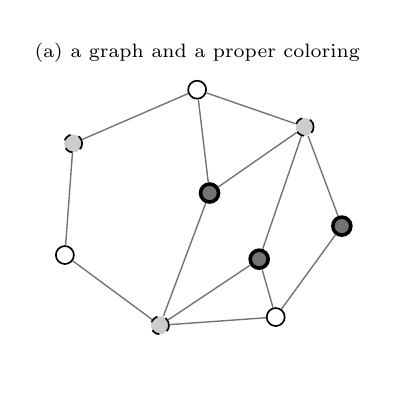
\begin{tikzpicture}[x=1.05cm, y=1.05cm,
  cA/.style={circle, draw=black, line width=0.6pt, fill=white, inner sep=0pt, minimum size=6.5pt},
  cB/.style={circle, draw=black, dashed, line width=0.6pt, fill=black!20, inner sep=0pt, minimum size=6.5pt},
  cC/.style={circle, draw=black, line width=1.3pt, fill=black!55, inner sep=0pt, minimum size=6.5pt},
  ed/.style={draw=black!55, line width=0.5pt}]
\useasboundingbox (-2.05,-1.95) rectangle (2.05,2.25);
\node[font=\scriptsize] at (0,1.95) {(a) a graph and a proper coloring};
\node[cA] (n1) at (0,1.5) {};
\node[cB] (n2) at (1.3,1.05) {};
\node[cC] (n3) at (1.75,-0.15) {};
\node[cA] (n4) at (0.95,-1.25) {};
\node[cB] (n5) at (-0.45,-1.35) {};
\node[cA] (n6) at (-1.6,-0.5) {};
\node[cB] (n7) at (-1.5,0.85) {};
\node[cC] (n8) at (0.15,0.25) {};
\node[cC] (n9) at (0.75,-0.55) {};
\draw[ed] (n1)--(n2); \draw[ed] (n2)--(n3); \draw[ed] (n3)--(n4);
\draw[ed] (n4)--(n5); \draw[ed] (n5)--(n6); \draw[ed] (n6)--(n7);
\draw[ed] (n7)--(n1); \draw[ed] (n1)--(n8); \draw[ed] (n2)--(n8);
\draw[ed] (n5)--(n8); \draw[ed] (n4)--(n9); \draw[ed] (n5)--(n9);
\draw[ed] (n2)--(n9);
\end{tikzpicture}
\end{minipage}\hfill
\begin{minipage}[b]{0.47\linewidth}
\centering
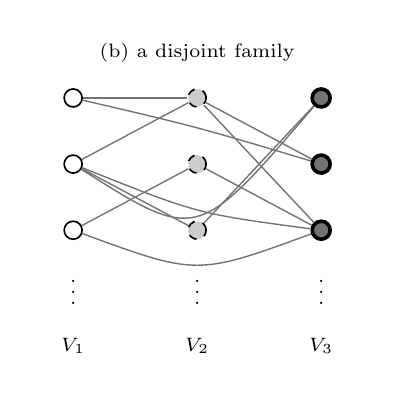
\begin{tikzpicture}[x=1.05cm, y=1.05cm,
  cA/.style={circle, draw=black, line width=0.6pt, fill=white, inner sep=0pt, minimum size=6.5pt},
  cB/.style={circle, draw=black, dashed, line width=0.6pt, fill=black!20, inner sep=0pt, minimum size=6.5pt},
  cC/.style={circle, draw=black, line width=1.3pt, fill=black!55, inner sep=0pt, minimum size=6.5pt},
  ed/.style={draw=black!55, line width=0.5pt}]
\useasboundingbox (-2.05,-1.95) rectangle (2.05,2.25);
\node[font=\scriptsize] at (0,1.95) {(b) a disjoint family};
\node[cA] (a1) at (-1.5,1.4) {}; \node[cA] (a2) at (-1.5,0.6) {}; \node[cA] (a3) at (-1.5,-0.2) {};
\node[cB] (b1) at (0,1.4) {};    \node[cB] (b2) at (0,0.6) {};    \node[cB] (b3) at (0,-0.2) {};
\node[cC] (c1) at (1.5,1.4) {};  \node[cC] (c2) at (1.5,0.6) {};  \node[cC] (c3) at (1.5,-0.2) {};
% Each drawn sequence realizes one item per position and asks for all of them,
% so the edge set is a union of transversal triangles: (a1,b1,c2), (a2,b3,c1),
% (a3,b2,c3), (a2,b1,c3). Every node lies in one, and no node is isolated or
% joined only inside its column. The A--C sides are bowed through the gaps
% between the middle column's nodes.
\draw[ed] (a1)--(b1); \draw[ed] (a2)--(b3); \draw[ed] (a3)--(b2);
\draw[ed] (a2)--(b1);
\draw[ed] (b1)--(c2); \draw[ed] (b3)--(c1); \draw[ed] (b2)--(c3);
\draw[ed] (b1)--(c3);
\draw[ed] (a1) .. controls (0,1.05) .. (c2);
\draw[ed] (a2) .. controls (0,-0.35) .. (c1);
\draw[ed] (a3) .. controls (0,-0.75) .. (c3);
\draw[ed] (a2) .. controls (0,0.0) .. (c3);
\node[font=\scriptsize] at (-1.5,-0.85) {$\vdots$};
\node[font=\scriptsize] at (0,-0.85) {$\vdots$};
\node[font=\scriptsize] at (1.5,-0.85) {$\vdots$};
\node[font=\scriptsize] at (-1.5,-1.6) {$V_1$};
\node[font=\scriptsize] at (0,-1.6) {$V_2$};
\node[font=\scriptsize] at (1.5,-1.6) {$V_3$};
\end{tikzpicture}
\end{minipage}
\caption{\textbf{Sizing as a coloring.} Nodes in (a) are the items a family can present, an edge joins two items some sequence asks for separately, and an assignment of items to features is a coloring, proper when no edge takes one color at both ends. The number of features the contract requires is the chromatic number, three here, and the triangle is what rules two out. Panel (b) is the disjoint family, one column per position: no edge lies inside a column, since symbols at one position never co-occur, so the columns grow as tall as the vocabularies $V_i$ are large while coloring by position stays proper however dense the edges between columns become. A sequence realizes one item per position and asks for all of them, so it contributes a triangle across the columns and every item a sequence realizes carries edges into every other position; the drawn edges are four such sequences. The chromatic number is the column count, and that coloring is the one a factorized map expresses at $\Slv$ parameters, levels as position digits.}
\label{fig:coloring}
\end{figure}

A contract bills two resources, and features are only the first: coloring the graph is a storage statement, and the width a cue must carry to select among the colors is the second (Appendix~\ref{apd:regimes}).


Whether the maps can serve a contract is a relation between two functions on the family. Write $\mathrm{addr}^{\mathrm{w}}$ and $\mathrm{addr}^{\mathrm{r}}$ for the addresses the two sides assign. A contract sending a query symbol $u$ to the stored symbol $\pi(u)$ is served when they agree:
\begin{align}
  \mathrm{addr}^{\mathrm{r}}(u) \;=\; \mathrm{addr}^{\mathrm{w}}\!\left(\pi(u)\right)
  \quad \text{for every } u ,
  \label{eq:agree}
\end{align}
Otherwise the read marginalizes densely over the digits it cannot fix, at an active-leaf count proportional to the matching instances, the bill attention pays for a multi-match query (Lemma~\ref{lem:agree}). Attention satisfies Eq.~\eqref{eq:agree} implicitly, $q \cdot k$ discriminating when the query carries what the key encoded.

The provisioning ratio $\alpha = \Nst / L$ is the dial a design sets. It says, roughly, how many features the head carries per token of context. What it buys is room for a coloring, and a coloring that exists settles neither that the map can express it nor that training finds one. The map realizes only the colorings that factor into a linear entmax classification per level. That is the hypothesis the grid of Section~\ref{sec:theorygrid} tests.

The number a contract requires is thus a functional of the distribution and the contract rather than a property of the head. What changes across families is how one comes to know it: a disjoint family asks for $L$ and a designer knows that in advance, where a shared family asks for a chromatic number only measurement returns. This paper measures neither (Appendix~\ref{apd:regimes}).

Sharing one feature between two symbols is safe when no retrieval map in the contract addresses one of them without the other. Two symbols that never co-occur may then share a feature for storage but not for retrieval, unless the cue the query addresses with covers everything that can land there (Appendix~\ref{apd:sharing}).

None of this asks the map to be computed per sequence, layer 1's family being the token vocabulary and depth supplying the dynamism thereafter (Appendix~\ref{apd:regimes}).

How $\Nst$ must scale with $L$ is a property of the sequences a task realizes rather than of $L$ alone, and the general sizing question is one this paper leaves open (Appendix~\ref{apd:regimes}).


Provisioning below the adversarial demand is a bet that the graph a design faces is smaller than the adversarial one, and Appendix~\ref{apd:regimes} gives the three things that shrink it.



\subsection{$\Nst = L$ as the adversarial contract}
\label{sec:corner}

At $\Nst = L$ the write side can be injective on instances, one color per occurrence, which covers the adversarial completion's demand whatever graph a sequence realizes. Every feature then holds one value, the failure mode above is structurally unavailable, and residual error lies on the read side alone. Softmax attention hardcodes this regime: its addresses are free, one per occurrence and injective by position, so its key map learns what a key encodes and never where it lands.


That regime is an entry fee. Real sequences are redundant, so provisioning $\Nst = \alpha L$ sizes the state to the information in a context rather than to its token count (Appendix~\ref{apd:regimes}).

Setting $\alpha < 1$ is thus a choice of what may alias: provisioning below the chromatic number forces edges to take one color at both ends (Figure~\ref{fig:coloring}). Entmax triage is what chooses the cheap ones, with leaf mass decay metering the turnover of the features that stay hot (Section~\ref{sec:decay}). Parity at $\Nst = L$ is the worst-case guarantee, and $\alpha$ is set from the costly-edge subgraph a distribution presents, which this paper leaves unmeasured.

